% Directory Structure

Class PixelSupervisorConfiguration Base helps to organize the output
directory, for example$:$ the output directories with runNumber
between 2000 and 2999 will be stored in directory
Run$\_$2000. PixelSupervisorConfiguration,
PixelFEDSupervisorConfiguration and PixelTKFECSupervisorConfiguration
are derived from this class. Using TBrowser of root, the final output
directory structure is showed in FIG.(\ref{fig:directory}). 

\subsection{Tree structure}\label{treestructure}

Tree structure is added in AddrssLevel, ROCUBEqualization,
VsfAndVHldDel, LinearityVsVsf, PHRange, VcThrCalDel, VcThr and CalDel
calibrations (among others). It helps to view some important information directly
through Histoviewer.

Two TTree pointers, tree and tree$\_$sum, are used to store
the information of "pass", and the
summary information, respectively. Table \ref{treeinformation} lists the pass
condition and summary information for the above
calibrations. The implementation of the tree structure is to declare
the struct in the header file of each kind of calibration. In the struct there must be a {\tt char} array to
store each ROC's name. This ensures that all the information can be
viewed by Histoviewer. 
The following code example is from
ROCUBEqualization calibration:
\begin{verbatim}
typedef struct branch{ 
    float pass; 
    char rocName[38];
   }; 
typedef struct branch_sum{
    float new_VIbias_DAC;
    float delta_VIbias_DAC;
    char rocName[38];
   };
\end{verbatim}

When using Histoviewer, the root output directory is as shown in
Fig.~\ref{rootdirectory}. The Detector Navigator view of HistoViewer
provides a graphical view of the detector, as illustrated in
Figures~\ref{passinfo} and \ref{summaryinfo}. These examples (from the
ROCUBEqualization calibration) show the values of pass state and the
new VIBias value selected by the calibration.



\begin{table}[htbp]
   \centering
\tiny{
    \caption{Pass condition and summary information stored in the trees. If the condition for failure is satisfied, then the `''Pass'' state is stored as 0 in the summary tree. Otherwise the ``Pass'' state is stored as 1.}
   \label{treeinformation}
  \begin{center}
 \begin{tabular}{lll}
 \hline \hline
 Calibration & Condition for Failure& Summary Information \\
   \hline
 Address Levels & Recommended Level $0^{\dagger}$ is less than UltraBlack high threshold &
 number of peaks, maximum peak RMS\\
  & or Number of ROC peaks found is not equal to $6$ & minimum peak separation, RMS of the black levels
 \\ \hline
ROC UB & The measured UB does not cross the target level &
 new VIBias value and change of VIBias \\ \hline
Vs & no hits found or no good Vsf found during scan &
 new Vsf value and the change of Vsf \\
 VHldDel &  &
 new VHldDel and its change \\ \hline 
LinearityVsVsf & no hits found or no good Vsf found during scan &
 new Vsf value and its change \\ \hline
PHRange & no hits found or no settings give PHInRange or &
 new VIbias$\_$PH, VOffsetOp and their changes \\
 & only one Vcal produces hits & new VIon and VOffsetRo and their changes \\ \hline
VcThrCalDel & there is not valid settings &  new VcThr, CalDel and their changes \\ \hline
VcThr & there is not valid VcThr &  new VcThr and its change \\ \hline
CalDel & there is not valid CalDel slope & new CalDel and its change \\ \hline 
Iana & new $\mathrm{Vana} \geq 249$ or maximum $\mathrm{Iana} < 25$ & new Vana, change in Vana, new Iana, \\
& & maximum Iana (fit Iana at $\mathrm{Vana}=250$), $\chi^2$ of the fit \\
\hline \hline
\end{tabular}
 \end{center}
}
 \end{table}


\begin{figure}
\begin{minipage}[htbp]{0.37\linewidth} % A minipage that covers half the
\centering
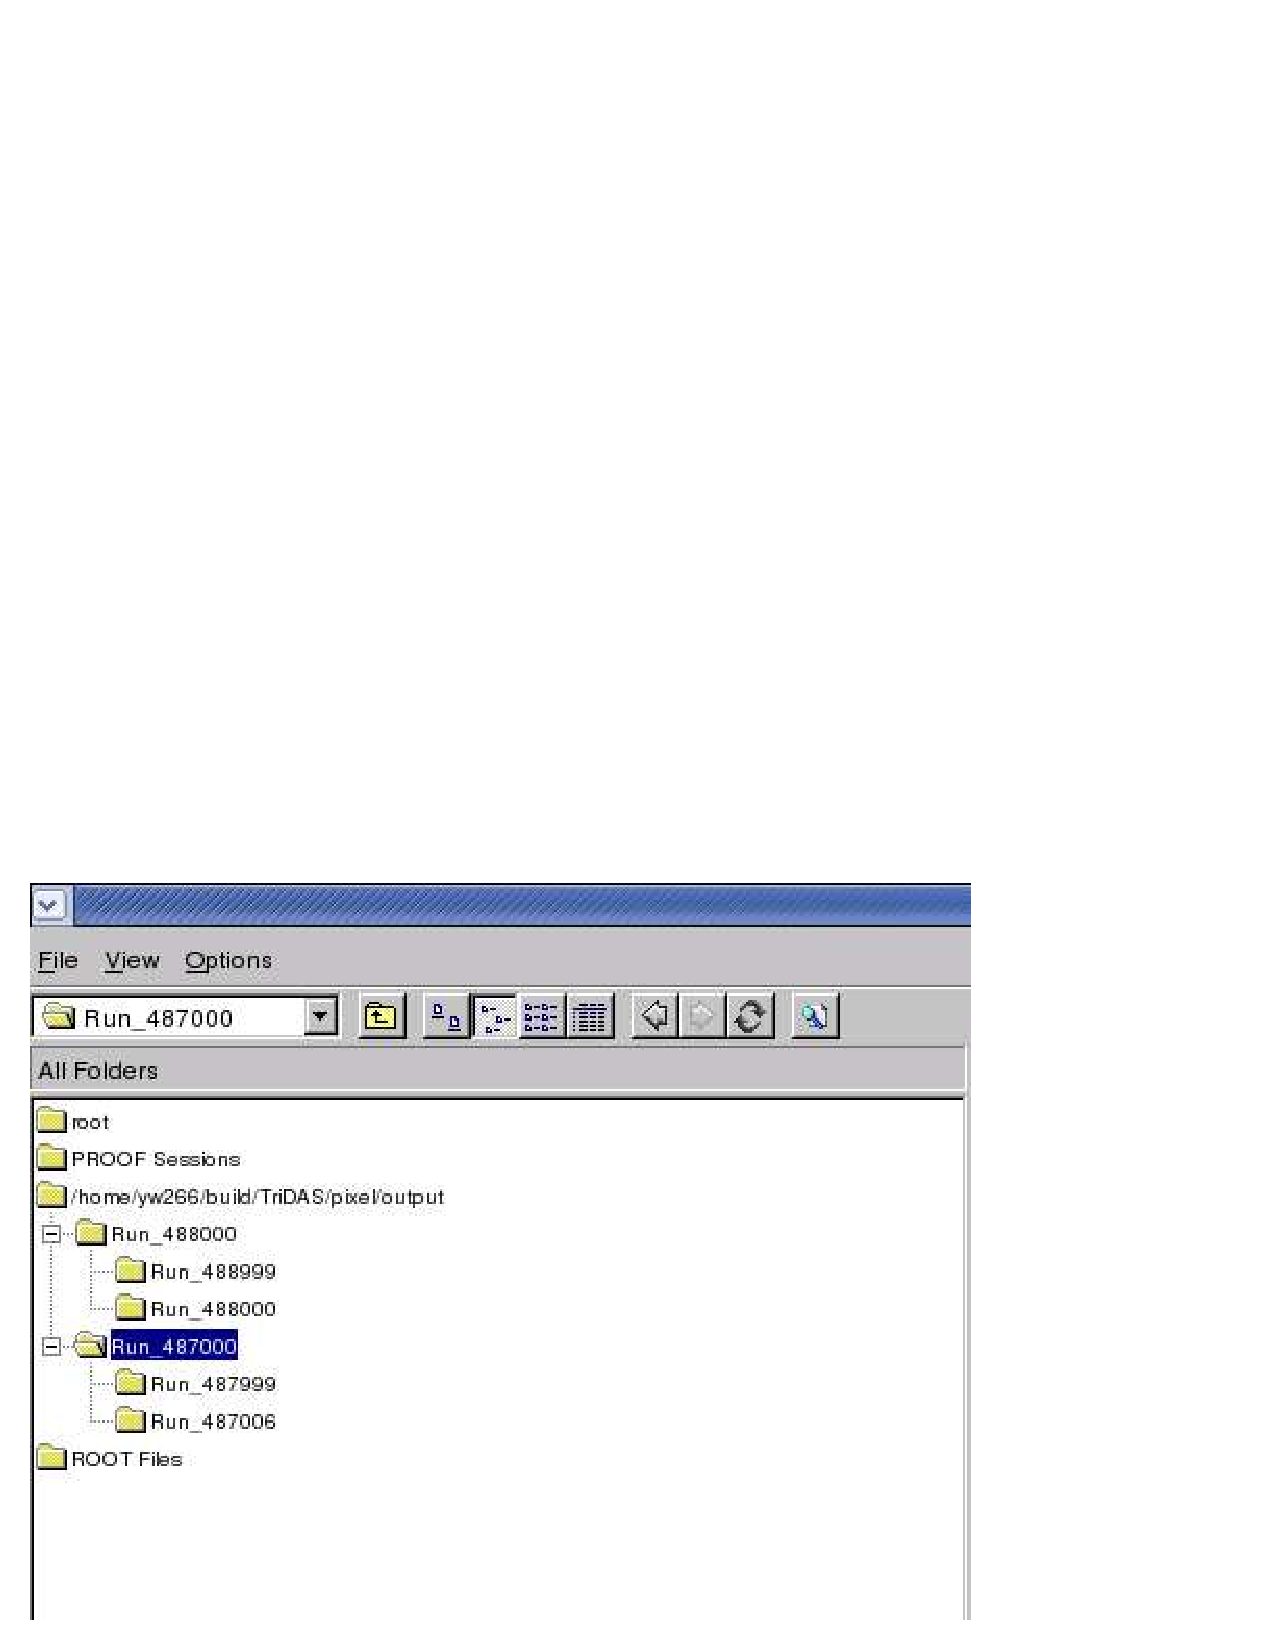
\includegraphics[width=7.5cm]{directory.pdf}
\caption{Output directory structure veiwing by ROOT.}
\label{fig:directory}
\end{minipage}
\hspace{0.5cm}
\begin{minipage}[htbp]{0.57\linewidth}
\centering
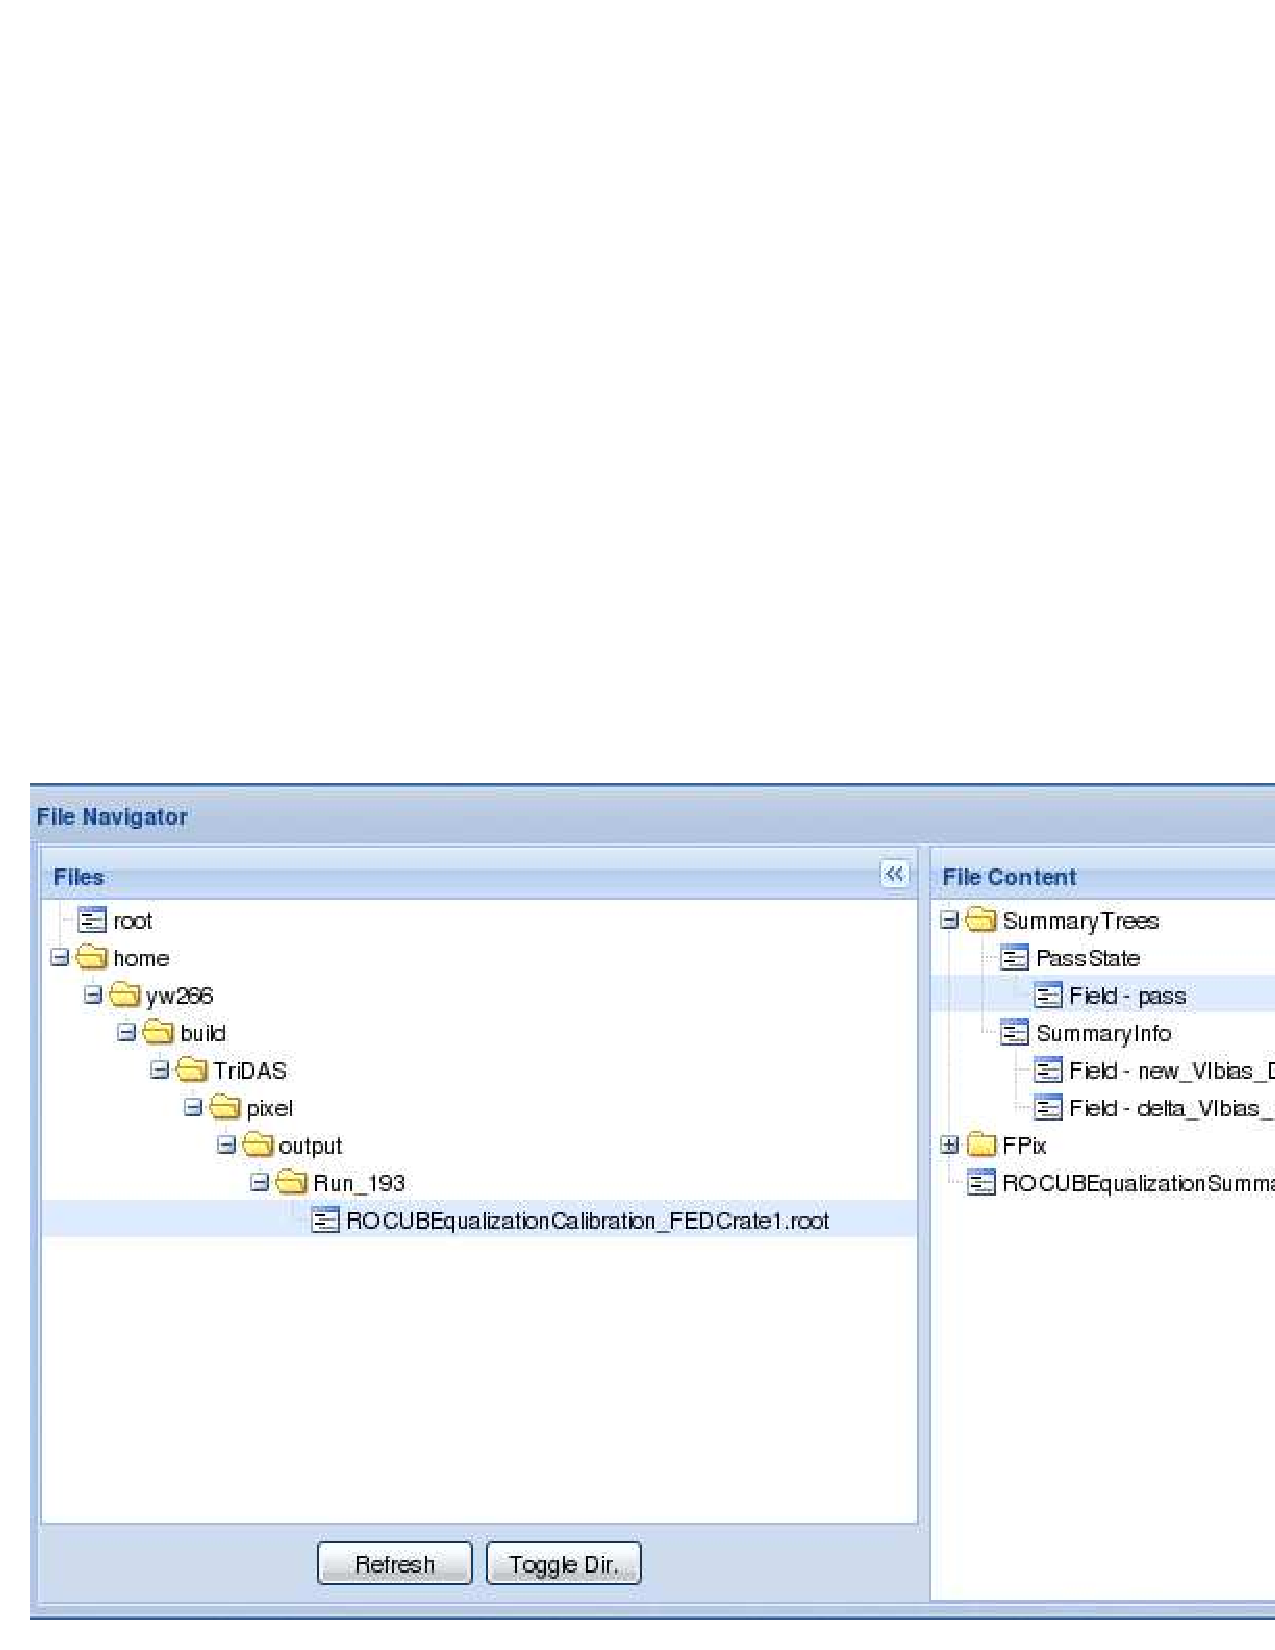
\includegraphics[width=9.5cm]{ROCUB_directory.pdf}
\caption{Output root directory structure veiwed by ROOT.}
\label{rootdirectory}
\end{minipage}
\end{figure}

\begin{figure}
\begin{minipage}[b]{0.47\linewidth} % A minipage that covers half the
\centering
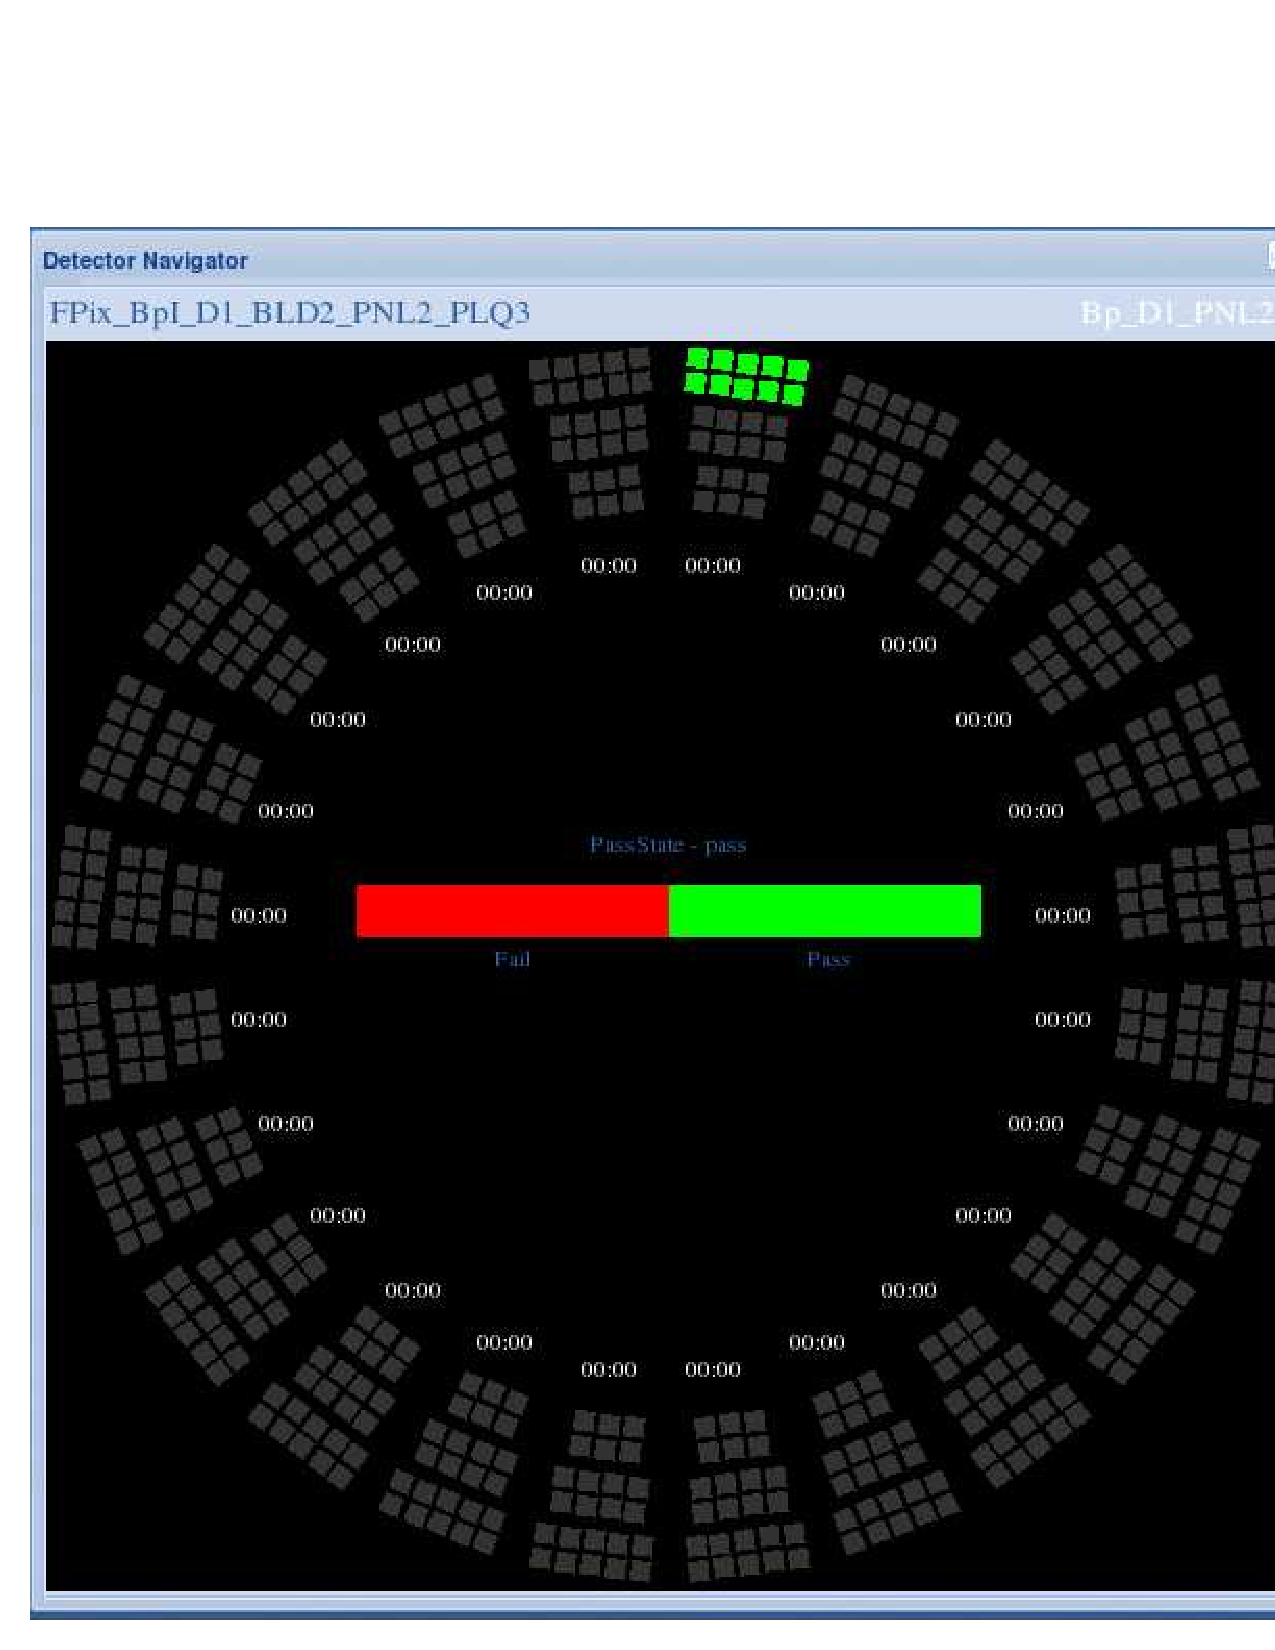
\includegraphics[width=5.5cm]{ROCUB_pass.pdf}
\caption{Pass information of ROCUBEqualization calibration viewed by histoviewer.}
\label{passinfo}
\end{minipage}
\hspace{0.5cm}
\begin{minipage}[b]{0.47\linewidth}
\centering
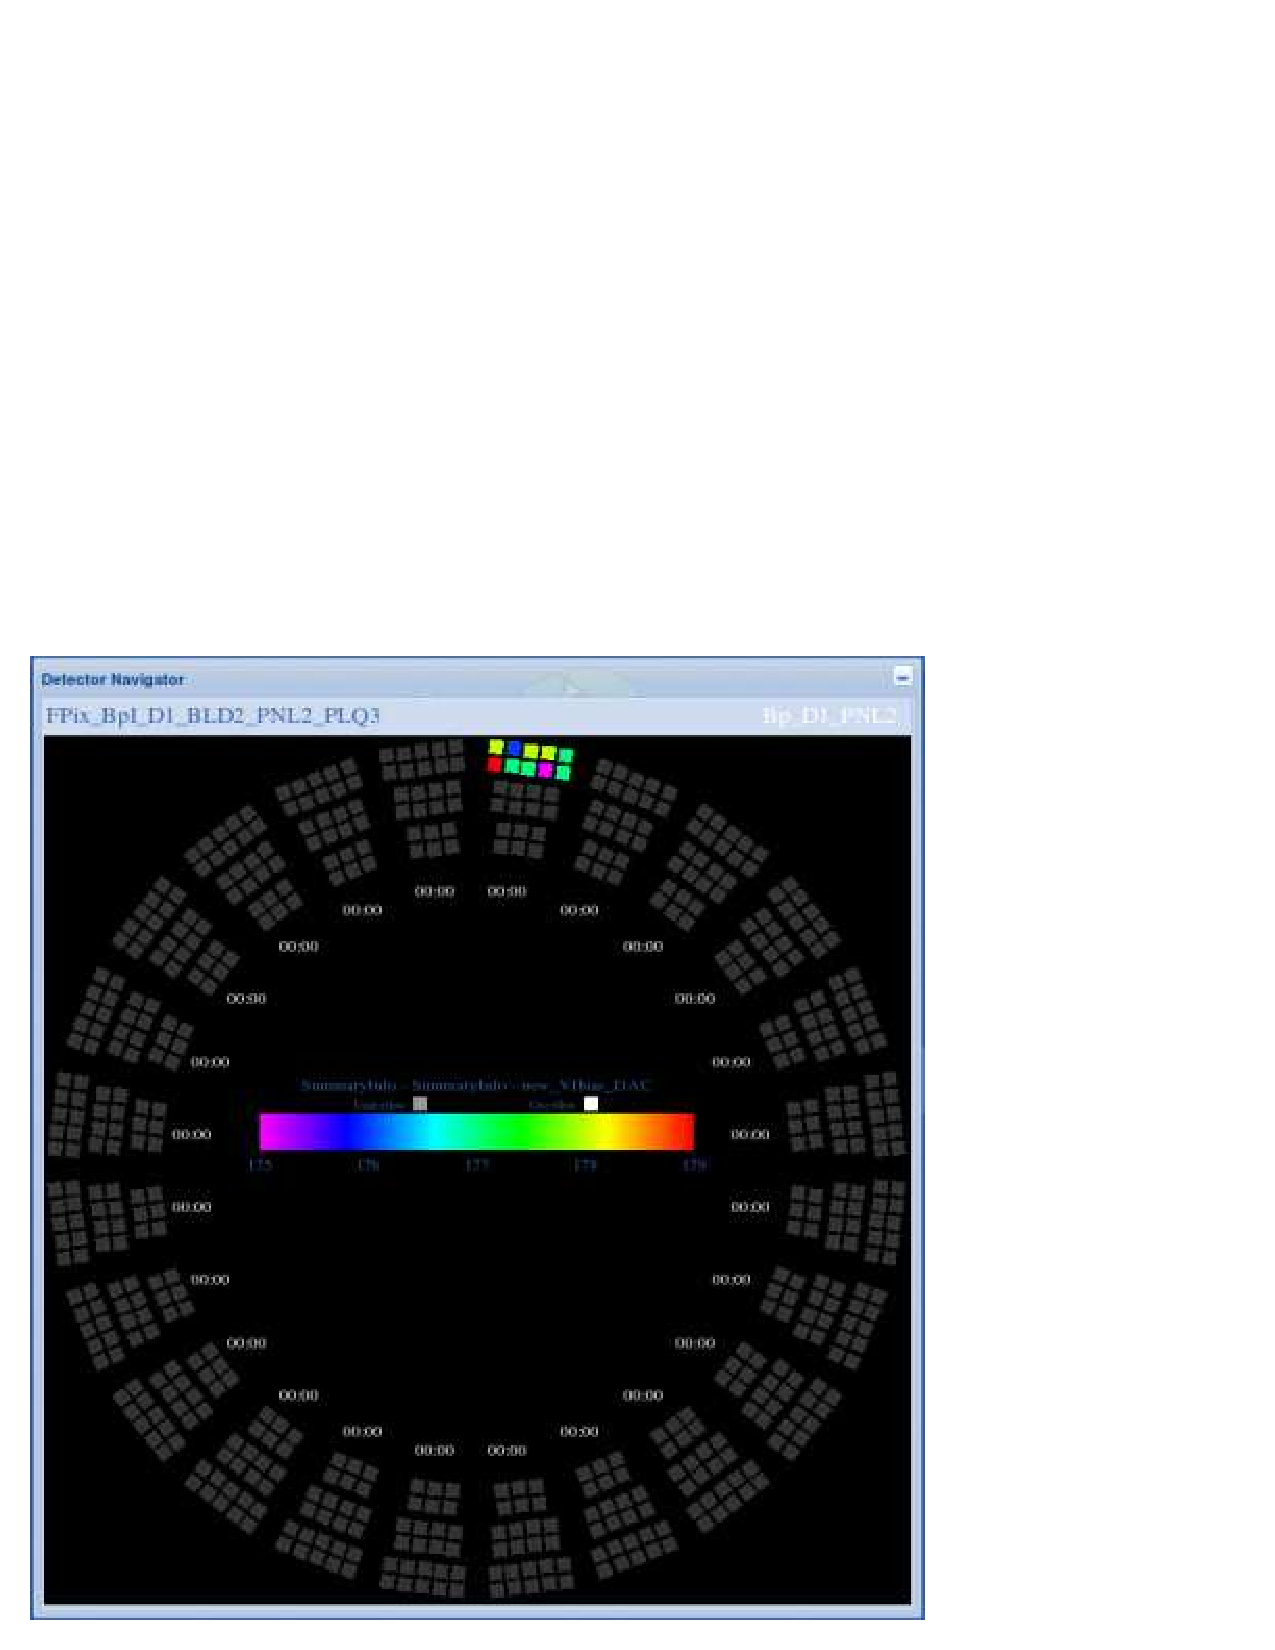
\includegraphics[width=8.5cm]{ROCUB_new_histoviewer.pdf}
\caption{New VIBias of ROCUBEqualization calibration veiwed by histoviewer.}
\label{summaryinfo}
\end{minipage}
\end{figure}

